\section{Phương pháp đề xuất}\label{sec:method}
\frame{\tableofcontents[currentsection]}

\subsection{Ý tưởng thực hiện luận văn}
\begin{frame}{Ý tưởng thực hiện luận văn}
    Luận văn kế thừa kết quả nghiên cứu của Lele Chen và cộng sự \cite{chen2019}
    \begin{figure}[H]
    \centering
    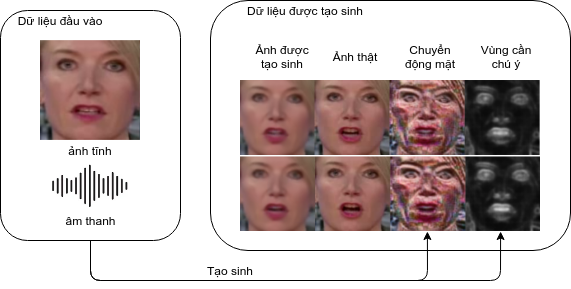
\includegraphics[width=12cm]{images/idea-small.png}
    \label{fig:idea}
    \caption{Ý tưởng tạo sinh hình ảnh từ ảnh gốc}
    \end{figure}
\end{frame}

\subsection{Cấu trúc tổng quát}

\begin{frame}{Cấu trúc tổng quát}
Hệ thống gồm có hai thành phần chính:
\begin{itemize}
    \item Mạng tạo sinh cột mốc gương mặt ($\Psi$)
    \item Hệ thống mạng GANs:
    \begin{itemize}
        \item Mạng tạo sinh video ($G$)
        \item Mạng phân biệt ($D$)
    \end{itemize}
\end{itemize}
\end{frame}

\begin{frame}{Cấu trúc tổng quát}
    \begin{figure}[H]
    \centering
    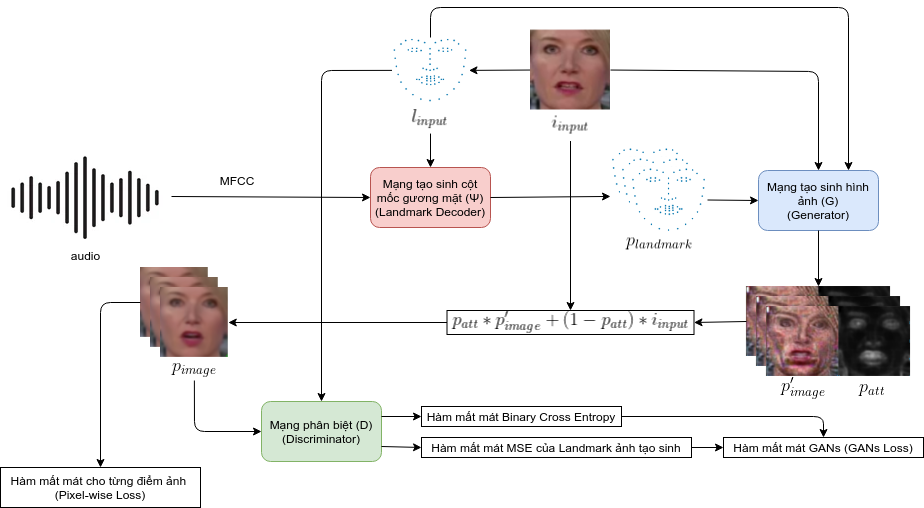
\includegraphics[width=12cm]{images/common_architecture.png}
    \label{fig:common_architecture}
    \caption{Cấu trúc tổng quát của hệ thống}
    \end{figure}
\end{frame}

\begin{frame}{Cấu trúc tổng quát}
    Hệ thống được mô hình hóa bằng công thức:
    \begin{equation}
        \begin{split}
        p_{landmark}(t) &= \Psi(l_{input}, mfcc(a(t)))\\
        p'_{image}(t), p_{att} &= G(i_{input}, l_{input}, p_{landmark})\\
        p_{image} &= p_{att}*p'_{image}+(1-p_{att})*i_{input}
        \end{split}
    \end{equation}
\end{frame}

\subsection{Tiền xử lý dữ liệu}
\begin{frame}{Tiền xử lý dữ liệu}
    Dữ liệu huấn luyện là các video với mặt người đang nói.
    \begin{itemize}
        \item Âm thanh: được trích xuất đặc trưng MFCC trước khi đưa vào mạng $\Psi$
        \item Hình ảnh: trích xuất và chuẩn hóa hình ảnh gương mặt sao cho mắt, mũi và miệng người nói trong các video có vị trí gần như nhau
        \item Cột mốc gương mặt: trích xuất và chuẩn hóa cột mốc gương mặt từ các video
    \end{itemize}
\end{frame}

\begin{frame}{Tiền xử lý dữ liệu}
    Đối với âm thanh
    \begin{figure}[H]
        \centering
        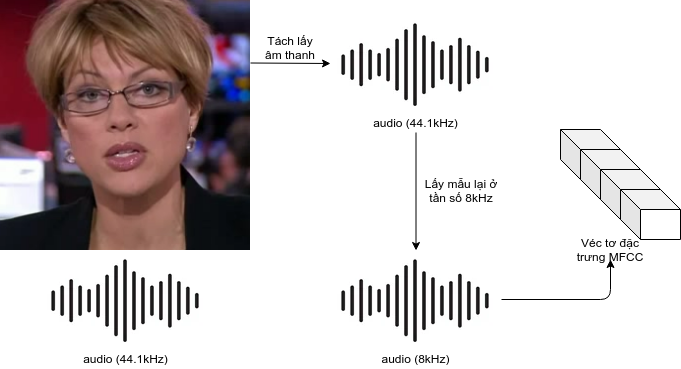
\includegraphics[width=11cm]{images/preprocess-audio.png}
        \label{fig:preprocess-audio}
        \caption{Tiền xử lý âm thanh}
    \end{figure}
\end{frame}

\begin{frame}{Tiền xử lý dữ liệu}
    Ta mong muốn đầu vào của mạng là một cột mốc gương mặt chung nhất và không bị ảnh hưởng bởi đặc điểm mặt người trên video. Vì vậy, ta cần tạo ra cột mốc gương mặt chuẩn bằng cách lấy trung bình cộng của nhiều cột mốc trong nhiều video khác nhau
    \begin{figure}[H]
        \centering
        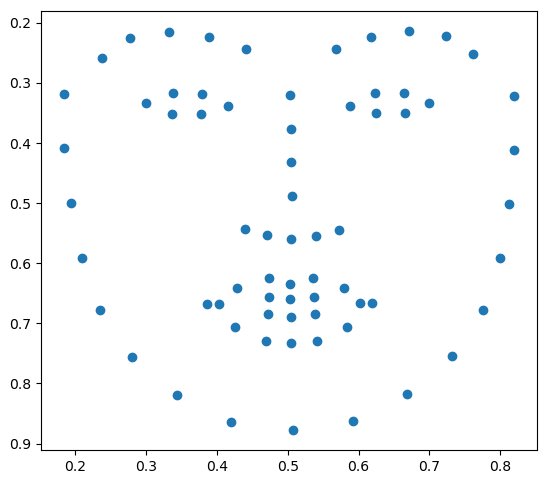
\includegraphics[width=6cm]{images/standard_landmark.png}
        \label{fig:standard_landmark}
        \caption{Cột mốc gương mặt chuẩn}
    \end{figure}
\end{frame}

\begin{frame}{Tiền xử lý dữ liệu}
    Với cách chuẩn hóa nêu trên, ta có thể đưa chuyển động của cột mốc gương mặt ban đầu lên cột mốc gương mặt chuẩn, với các góc độ quay khác nhau của video và loại bỏ đặc điểm gương mặt người nói
    \begin{figure}[H]
        \centering
        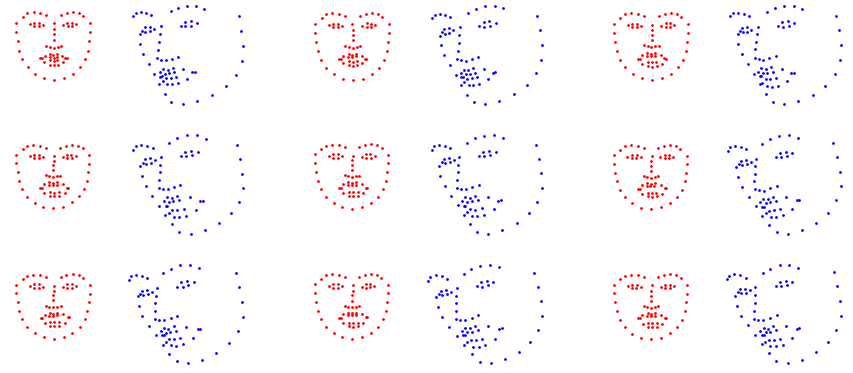
\includegraphics[width=11cm]{images/standardize_landmark.png}
        \label{fig:standardize_landmark}
        \caption{Kết quả chuẩn hóa cột mốc gương mặt. Cột mốc ban đầu (xanh), chuẩn hóa (đỏ)}
    \end{figure}
\end{frame}

\begin{frame}{Tiền xử lý dữ liệu}
    Với cách chuẩn hóa hình ảnh trên, ta có thể đưa mắt, mũi, miệng người nói trong video về một vị trí gần như nhau trong mọi video
    \begin{figure}[H]
        \centering
        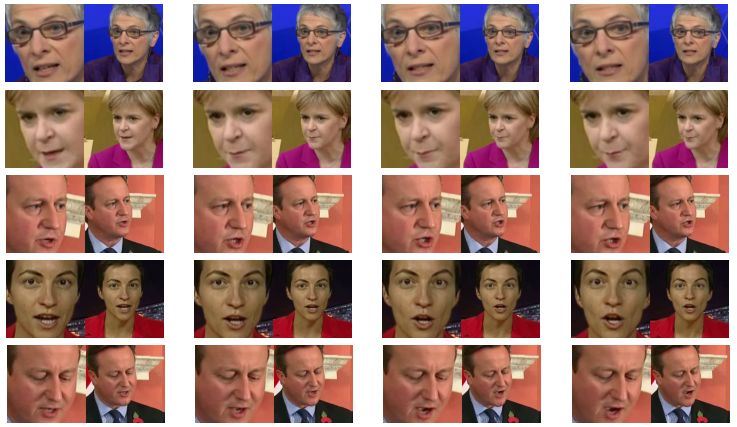
\includegraphics[width=10cm]{images/preprocess-image.png}
        \label{fig:preprocess-image}
        \caption{Kết quả chuẩn hóa hình ảnh}
    \end{figure}
\end{frame}

\subsection{Cấu trúc chi tiết}
\begin{frame}{Cấu trúc bộ giải mã cột mốc gương mặt (Landmark Decoder)}
    \begin{figure}[H]
        \centering
        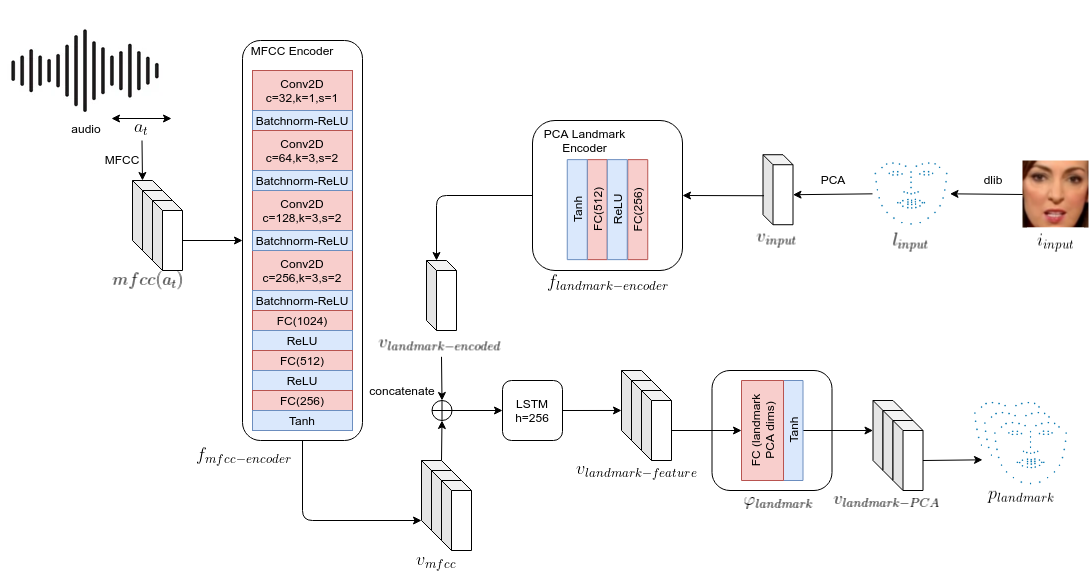
\includegraphics[width=13cm]{images/landmark_decoder.png}
        \label{fig:landmark_decoder}
        \caption{Cấu trúc bộ giải mã cột mốc gương mặt (Landmark Decoder)}
    \end{figure}
\end{frame}

\begin{frame}{Cấu trúc bộ giải mã cột mốc gương mặt (Landmark Decoder)}
    Landmark Decoder được mô hình hóa bằng công thức:
    \begin{equation}
        \begin{split}
        v_{landmark-encoded} &= f_{landmark-encoder}(PCA(l_{input}))\\
        v_{mfcc}(t) &= f_{mfcc-encoder}(mfcc(a_t))\\
        v_{landmark-feature} &= LSTM(v_{landmark-encoded} \oplus v_{mfcc})\\
        p_{landmark} &= PCA_R(\varphi_{landmark}(v_{landmark-feature}))
        \end{split}
    \end{equation}
\end{frame}

\begin{frame}{Cấu trúc bộ tạo sinh hình ảnh (Generator)}
    \begin{figure}[H]
        \centering
        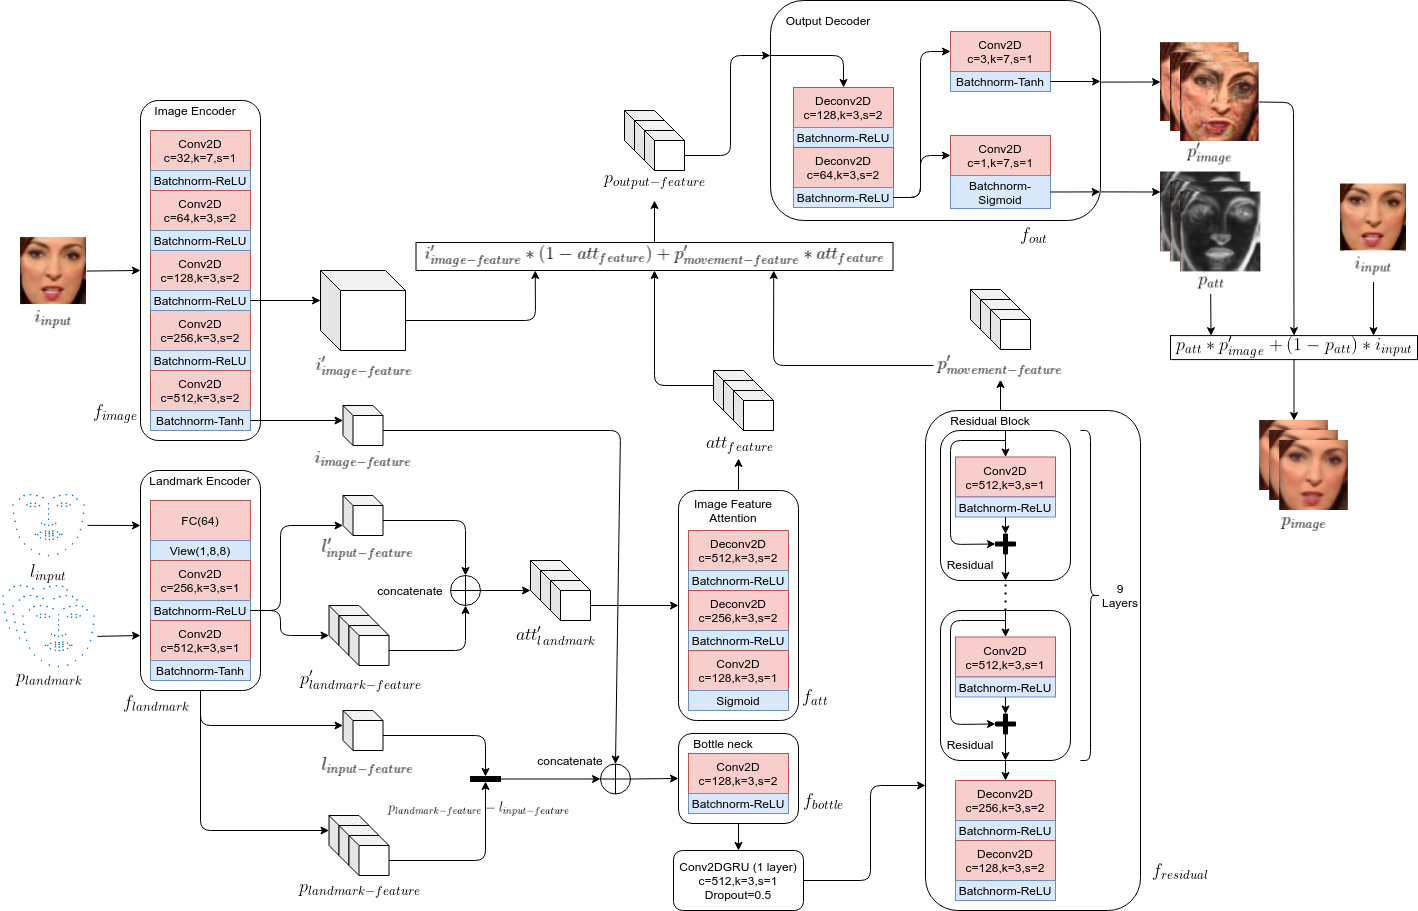
\includegraphics[width=10.5cm]{images/generator.png}
        \label{fig:generator}
        \caption{Cấu trúc bộ tạo sinh hình ảnh (Generator)}
    \end{figure}
\end{frame}

\begin{frame}{Cấu trúc bộ tạo sinh hình ảnh (Generator)}
    Generator được mô hình hóa bằng công thức:
    \begin{equation}
        \begin{split}
        i'_{image-feature}, i_{image-feature} &= f_{image}(i_{input})\\
        l'_{input-feature}, l_{input-feature} &= f_{landmark}(l_{input})\\
        p'_{landmark-feature}, p_{landmark-feature} &= f_{landmark}(p_{landmark})\\
        p'_{movement-feature}(t) &= f_{residual}(CRNN(f_{bottle}(i_{image-feature} \\
        &\oplus (p_{landmark-feature}(t)-l_{input-feature}))))\\
        att_{feature}(t) &= f_{att}(p'_{landmark-feature}(t) \oplus l'_{input-feature})\\
        p_{output-feature}(t) &= i'_{image-feature}*(1-att_{feature}(t))+\\
        &p'_{movement-feature}(t)*att_{feature}(t)\\
        p_{att}(t), p'_{image}(t) &= f_{out}(p_{output-feature}(t))\\
        p_{image}(t) &= p_{att}(t)*p'_{image}(t)+(1-p_{att}(t))*i_{image}
        \end{split}
    \end{equation}
\end{frame}

\begin{frame}{Cấu trúc bộ phân biệt (Discriminator)}
    \begin{figure}[H]
        \centering
        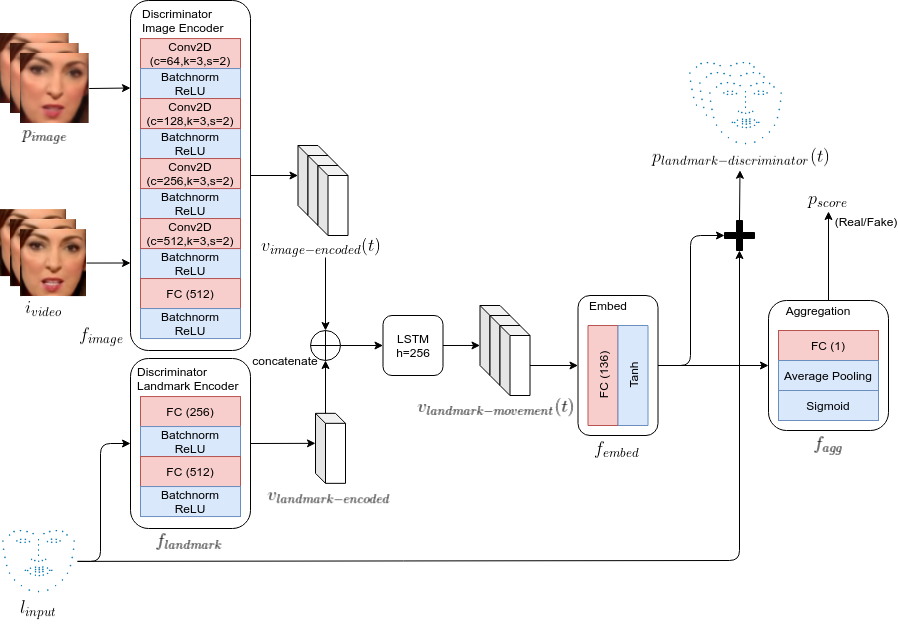
\includegraphics[width=10cm]{images/discriminator.png}
        \label{fig:discriminator}
        \caption{Cấu trúc bộ phân biệt (Discriminator)}
    \end{figure}
\end{frame}

\begin{frame}{Cấu trúc bộ phân biệt (Discriminator)}
    Discriminator được mô hình hóa bằng công thức:
    \begin{equation}
        \begin{split}
        v_{image-encoded}(t) &= f_{image}(p_{image}(t)|i_{video}(t))\\
        v_{landmark-encoded} &= f_{landmark}(l_{input})\\
        v_{landmark-movement} &= LSTM(v_{image-encoded} \oplus v_{landmark-encoded})\\
        p_{landmark-discriminator}(t) &= f_{embed}(v_{landmark-movement}(t) + l_{input})\\
        p_{score} &= f_{agg}(f_{embed}(v_{landmark-movement}))
        \end{split}
    \end{equation}
\end{frame}

\subsection{Hàm mất mát}

\begin{frame}{Hàm mất mát cho từng pixel}
    \begin{equation}
        \mathcal{L}_{pix} = \frac{1}{T}\sum^T_{t=1}||(i_{video}(t)-p_{image}(t))*(p_{att}(t)+\beta)||_1
    \end{equation}
    
    Trong đó:
    \begin{itemize}
        \item \textbf{$i_{video}(t)$}: khung hình tại thời điểm $t$ của video gốc
        \item \textbf{$p_{image}(t)$}: hình ảnh được tạo sinh tại thời điểm $t$
        \item \textbf{$p_{att}(t)$}: mặt nạ chú ý được dự đoán tại thời điểm $t$
        \item \textbf{$\beta$}: một hằng số để đảm bảo tất cả các điểm trên ảnh đều được học, ta chọn $\beta = 0.5$ 
    \end{itemize}
    
\end{frame}

\begin{frame}{Hàm mất mát GANs cho bộ phân biệt}
    \begin{equation}
        \begin{split}
        \mathcal{L}_{gans-dis} = &\mathbb{E}_{l_{input},i_{video}}[logD_s(l_{input},i_{video})]\\
        +&\mathbb{E}_{l_{input},i_{input},p_{landmark}}[log(1-D_s(l_{input},G(l_{input},i_{input},p_{landmark})))]
        \end{split}
    \end{equation}
    Trong đó:
    \begin{itemize}
        \item \textbf{$l_{input},i_{input},p_{landmark},i_{video}$}: đã được giải thích ở các phần trên
        \item \textbf{$D_s$}: Mạng phân biệt với đầu ra là xác suất ảnh là ảnh thật
        \item \textbf{$G$}: Mạng tạo sinh hình ảnh
    \end{itemize}
\end{frame}

\begin{frame}{Hàm mất mát GANs cho bộ phân biệt}
\begin{equation}
    \begin{split}
    \mathcal{L}_{gans-landmark} = &||(D_l(l_{input},G(l_{input},i_{input},p_{landmark})) - l_{orig})*M_l||^2_2\\
    +&||(D_l(l_{input},i_{video}) - l_{orig})*M_l||^2_2\\
    \end{split}
\end{equation}

    Trong đó:
    \begin{itemize}
        \item \textbf{$l_{input},i_{input},p_{landmark},i_{video}$}: đã được giải thích ở các phần trên
        \item \textbf{$D_l$}: Mạng phân biệt với đầu ra là cột mốc gương mặt trên ảnh được tạo sinh
        \item \textbf{$G$}: Mạng tạo sinh hình ảnh
        \item \textbf{$l_{original}$}: Cột mốc gương mặt được trích xuất nguyên gốc từ video $i_{video}$
        \item \textbf{$M_l$}: mặt nạ nhằm chú ý nhiều hơn vào cột mốc gương mặt vùng miệng, theo đó, sai số của cột mốc ở vùng miệng có hệ số 100, trong khi các vùng khác là 1.
    \end{itemize}
\end{frame}

\begin{frame}{Hàm mất mát tổng}
    \begin{equation}
        \begin{split}
        \mathcal{L}_{gans} = &\mathcal{L}_{gans-dis} + \mathcal{L}_{gans-landmark}\\
        \mathcal{L} = &\mathcal{L}_{gans} + \lambda*\mathcal{L}_{pix}
        \end{split}
    \end{equation}
    Với $\lambda = 10$
\end{frame}
